% Part   : Distribution
% Chapter: Anaconda Header
% Section: Identity
% ------------------------------------------------------------
% $Id$
% ------------------------------------------------------------

\begin{figure}[!hbp]
\hrulefill
\begin{verbatim}
trunk/Identity/Themes/$THEME/Distro/Anaconda/Header/
|-- img
|   |-- 3
|   |   |-- anaconda_header.png.png
|   |-- 4
|   |-- 5
|   `-- ... more major releases
|-- render.sh
`-- tpl
    `-- anaconda_header.png.svg
\end{verbatim}
\hrulefill
\caption{Anaconda header identity's framework.%
   \label{fig:Distribution:Anaconda:Header:Identity}}
\end{figure}

\subsection{Designs Templates}
\hypertarget{sec:Distribution:Anaconda:Header:Identity:Templates}{}
\label{sec:Distribution:Anaconda:Header:Identity:Templates}

\begin{itemize}
\item trunk/Identity/Themes/\$THEME/Distro/Anaconda/Header/tpl
\end{itemize}

\subsection{Design Models}

\begin{itemize}
\item trunk/Identity/Models/Tpl/Distro/Anaconda/Header/
\item trunk/Identity/Models/Img/Distro/Anaconda/Header/
\end{itemize}

\begin{figure}[!hbp]
\begin{center}
\fbox{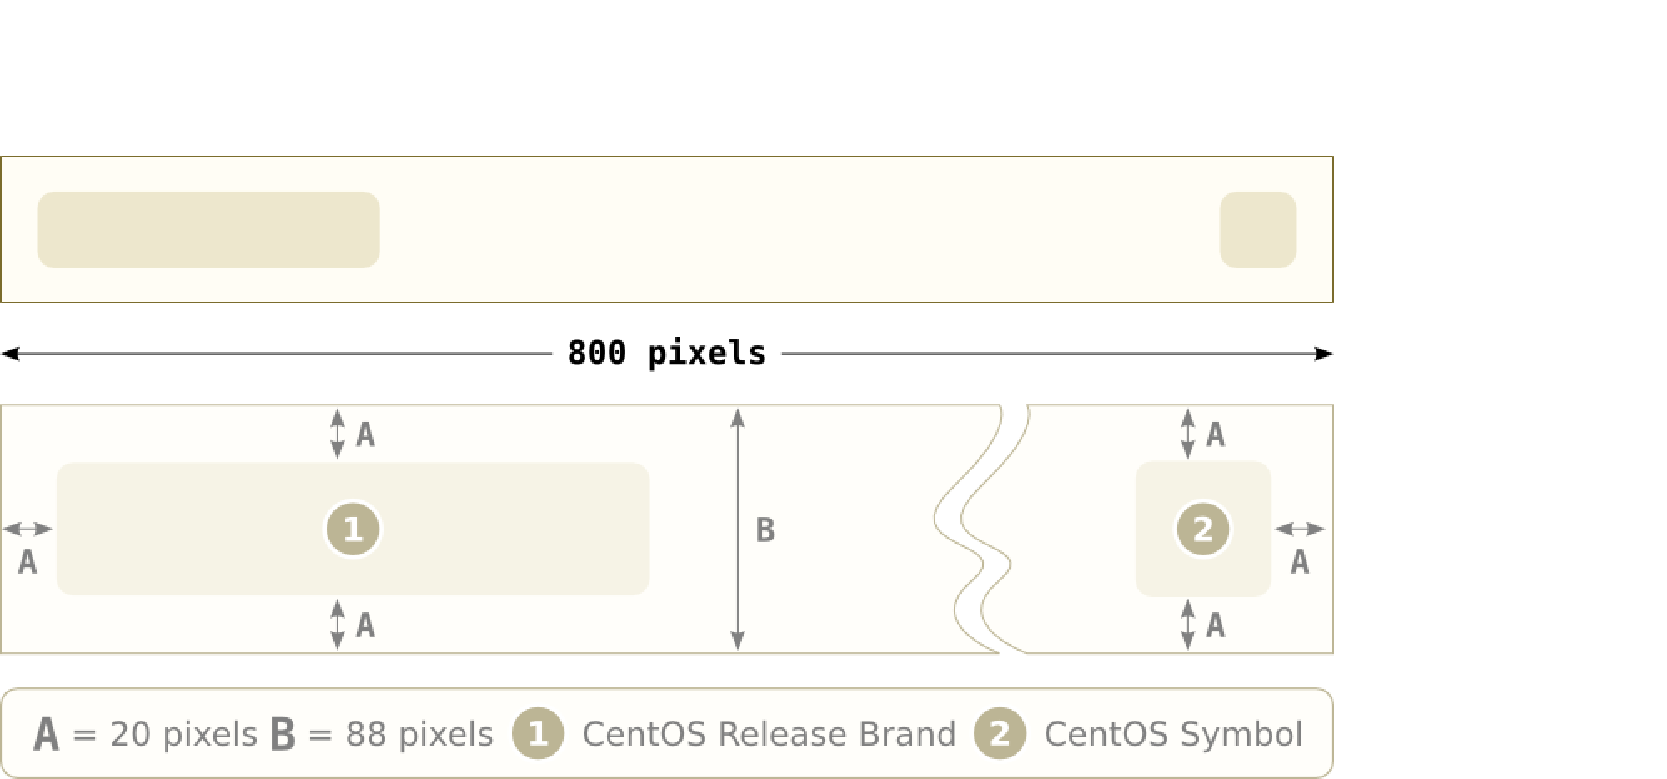
\includegraphics[width=0.8\textwidth]{%
   /home/centos/artwork/trunk/Identity/Models/Img/en/Distro/Anaconda/Header/fig-1-anaconda_header.pdf}} 
\end{center}
\caption{Anaconda header design model.% 
   \label{fig:Distribution:Anaconda:Header:Models:Fig1}}
\end{figure}

\begin{figure}[!hbp]
\begin{center}
\fbox{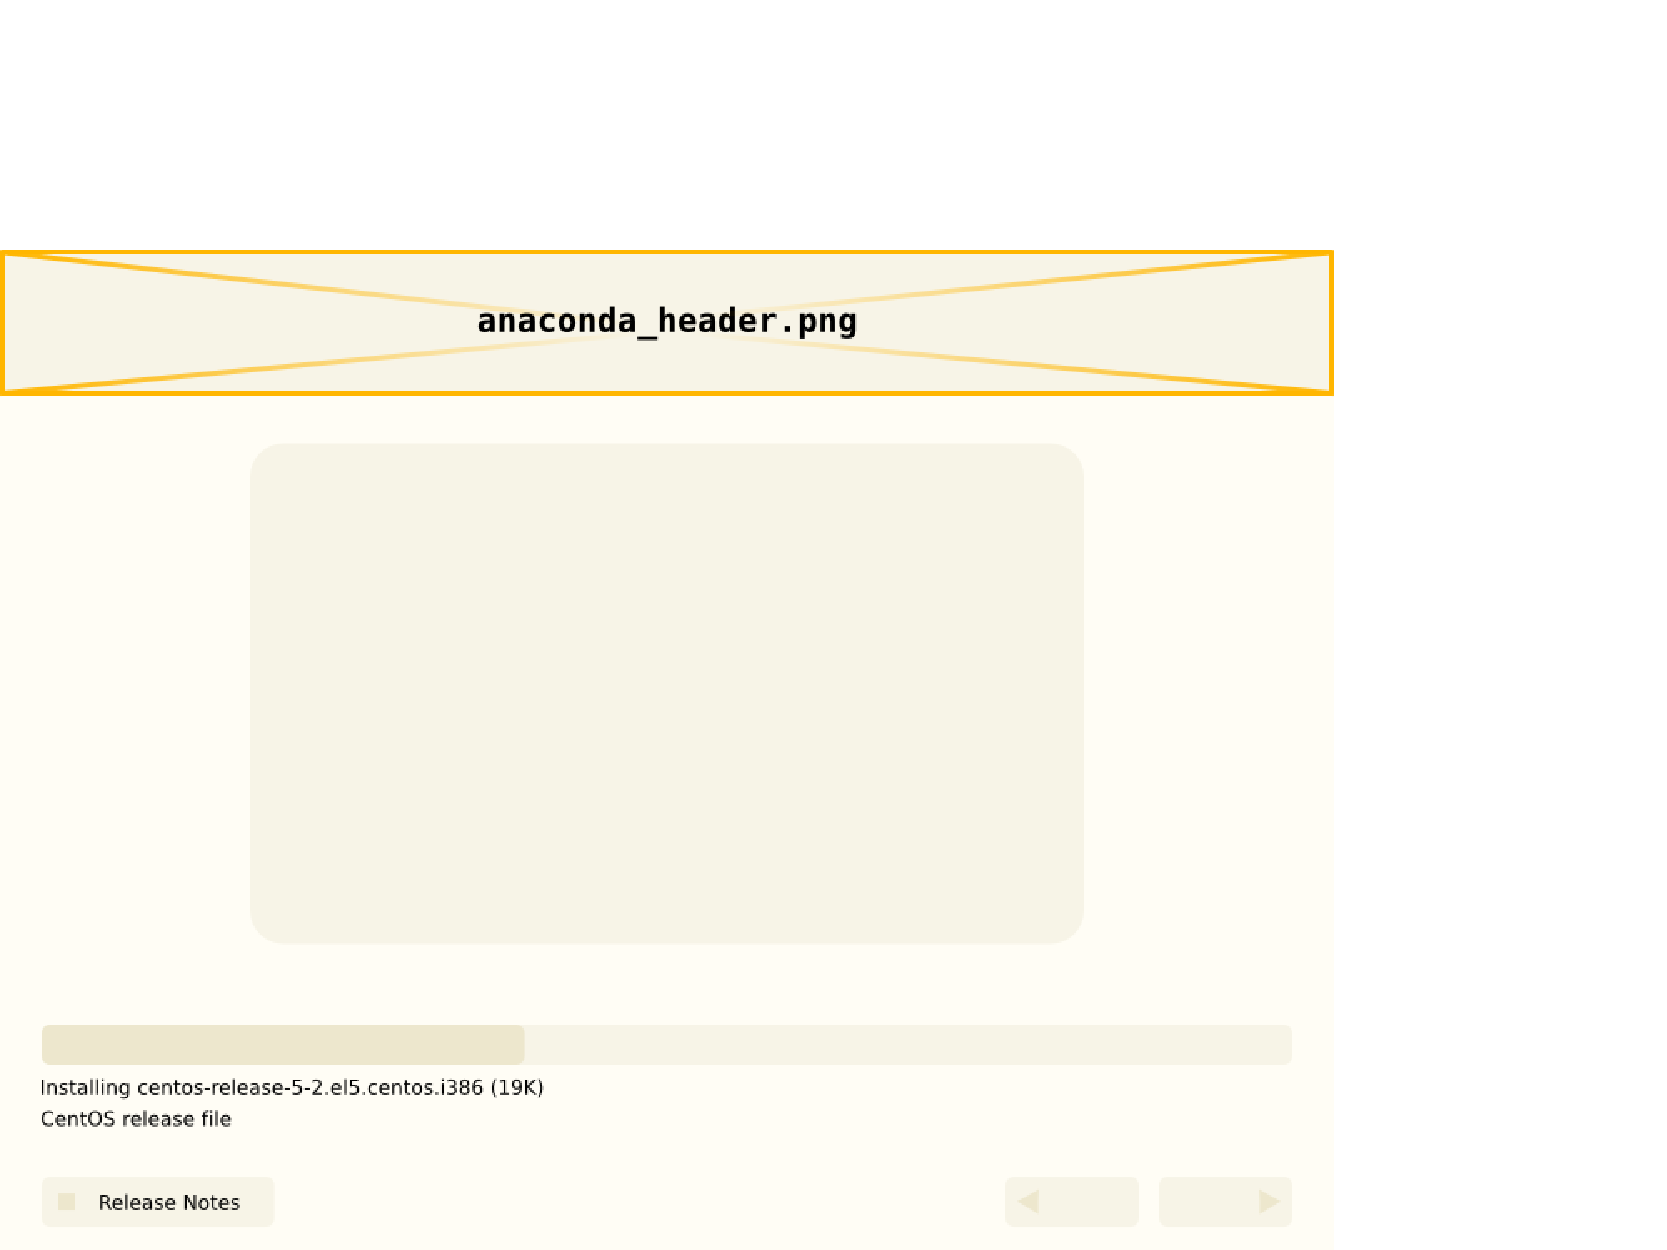
\includegraphics[width=0.8\textwidth]{%
   /home/centos/artwork/trunk/Identity/Models/Img/en/Distro/Anaconda/Header/fig-2-anaconda_header.pdf}} 
\end{center}
\caption{Anaconda header position in the screen.% 
   \label{fig:Distribution:Anaconda:Header:Models:Fig2}}
\end{figure}

\subsection{Image Files}
\hypertarget{sec:Distribution:Anaconda:Header:Identity:Images}{}
\label{sec:Distribution:Anaconda:Header:Identity:Images}

\begin{itemize}
\item \texttt{anaconda\_header.png}: base image format.
\end{itemize}

\subsection{Image Files Rendering}
\hypertarget{sec:Distribution:Anaconda:Header:Identity:Issues}{}
\label{sec:Distribution:Anaconda:Header:Identity:Issues}
\fbox{\texttt{./render.sh}}
\fbox{\texttt{./render.sh '5'}}
\fbox{\texttt{./render.sh '(3|4|5)'}}

\subsection{Color Limitations}
\hypertarget{sec:Distribution:Anaconda:Header:Identity:Colors}{}
\label{sec:Distribution:Anaconda:Header:Identity:Colors}

Anaconda Header does not have color limitations. 

\subsection{Issues}
\hypertarget{sec:Distribution:Anaconda:Header:Issues}{}
\label{sec:Distribution:Anaconda:Header:Issues}

No one known.
